\section{Experimental Evaluation}

\subsection{Datasets}
Our experimental framework evaluates TURRET OS across two primary datasets, as detailed in \Cref{tab:dataset_stats}:
\begin{itemize}
    \item \textbf{D3 TSEC (Synthetic Corpus)}: A seeded, deterministic synthetic corpus comprising 500 users over 365 days, yielding 141,725 activity records and 14 malicious actors (1.91\% positive rate).
    \item \textbf{D5 Synthetic-Tenant Pilot}: A 90-day lab deployment pilot comprising 35 users, 2,446 activity records, and 3 tagged insider scenarios (3.80\% positive rate).
    \item \textbf{D1/D2 CERT Benchmarks}: CERT r6.2 and r4.2 datasets require Carnegie Mellon University SEI Data Use Agreement (DUA) authorization and are explicitly footnoted in \Cref{tab:dataset_stats}.
\end{itemize}

\begin{table}[htbp]
\caption{Dataset Statistics across Evaluation Corpora.}
\label{tab:dataset_stats}
\centering
\small
\begin{tabularx}{\linewidth}{X r r r r}
\toprule
\textbf{Dataset} & \textbf{Users} & \textbf{Records} & \textbf{Actors} & \textbf{Pos. Rate (\%)} \\
\midrule
D3 TSEC (synthetic) & 500 & 141,725 & 14 & 1.91\% \\
D5 Synthetic-Tenant & 35 & 2,446 & 3 & 3.80\% \\
D1 CERT r6.2 & \multicolumn{4}{c}{\textit{Requires SEI DUA}} \\
D2 CERT r4.2 & \multicolumn{4}{c}{\textit{Requires SEI DUA}} \\
\bottomrule
\end{tabularx}
\end{table}

\subsection{Detection Performance Against Published Baselines}
\Cref{tab:detection_performance} compares TURRET OS against 14 published baselines. To avoid metric-type mixing, literature baseline figures are reported under their original published metric type with explicit provenance annotations. On D3 TSEC, TURRET OS achieves an uncalibrated ROC-AUC of 0.9983, a calibrated best F1-score of 0.9747, an F1-score of 0.8813 at a strict 0.5\% FPR operating point, an MCC of 0.9732, and an operational time-to-detect of $<0.1$ minutes.

\begin{table*}[htbp]
\caption{Detection Performance Comparison vs. Published Baselines (Explicit Provenance).}
\label{tab:detection_performance}
\centering
\footnotesize
\begin{tabularx}{\textwidth}{X l c c c X}
\toprule
\textbf{System} & \textbf{Reported Metric} & \textbf{Reported Val.} & \textbf{F1@0.5\%FPR} & \textbf{TTD (min)} & \textbf{Provenance Citation} \\
\midrule
\textbf{TURRET OS (ours)} & ROC-AUC / F1@0.5\% & \textbf{0.9983 / 0.9747} & \textbf{0.8813} & \textbf{0.0} & Calculated on D3 TSEC (Calibrated) \\
E-Watcher \citep{wei2024ewatcher} & ROC-AUC / Acc & 0.9848 & NR & NR & Wei et al. (2024) IEEE TIFS (Accuracy 98.48\%) \\
Le \& Zincir-Heywood \citep{le2020insider} & ROC-AUC & 0.9200 & NR & 14.0 & Le \& Zincir-Heywood (2020), TTD=14min \\
DTGI \citep{ga02023dtgi} & ROC-AUC & 0.9100 & NR & NR & Gao et al. (2023) IEEE TDSC, Table II \\
TGCN-DA \citep{li2023tgcnda} & ROC-AUC & 0.9500 & NR & NR & Li et al. (2023) Computers \& Security \\
MEWRGNN \citep{xiao2022mewrgnn} & ROC-AUC & 0.9400 & NR & NR & Xiao et al. (2022) Pattern Recognition \\
SENTINEL \citep{xiao2024sentinel} & ROC-AUC & 0.9300 & NR & NR & Xiao et al. (2024) IEEE TIFS \\
Vidhya spatio-temporal \citep{vidhya2024spatiotemporal} & ROC-AUC & 0.9100 & NR & NR & Vidhya et al. (2024), Table V \\
KRYSTAL KG \citep{kurniawan2022krystal} & ROC-AUC & 0.8900 & NR & NR & Kurniawan et al. (2022), Table II \\
MetaShield \citep{hamid2025metashield} & ROC-AUC & 0.8600 & NR & NR & Hamid \& Safizada (2025), Table I \\
Exif2Vec \citep{umair2024exif2vec} & ROC-AUC & 0.8200 & NR & NR & Umair et al. (2024), Table III \\
Yasenenko image-meta \citep{yasenenko2025imagemeta} & ROC-AUC & 0.7600 & NR & NR & Yasenenko (2025), Table I \\
DFR-BUST \citep{shoderu2025dfrbust} & NR & NR & NR & NR & Shoderu et al. (2025), Readiness Matrix \\
PS0 provenance+rules \citep{mavroeidis2018ps0} & ROC-AUC & 0.7200 & 0.6100 & NR & Mavroeidis (2018), F1@0.5\% FPR reported \\
Static prediction \citep{le2019static} & ROC-AUC & 0.6500 & NR & NR & Le (2019), Table I \\
\bottomrule
\end{tabularx}
\end{table*}

\subsection{Layer Ablation Study and Leakage Audit}
\Cref{tab:ablation} details the layer-by-layer ablation study evaluated across 5 random seeds (42, 43, 44, 45, 46). To verify that graph topology adds genuine discriminative signal rather than feature leakage, we evaluate an L1-only classifier on a strict chronological split (AUC 0.8502 $\pm 0.0$). Adding Layer 2 knowledge graph representation boosts ROC-AUC to 0.9918 ($\pm 0.0031$), confirming that structural provenance relationships provide a $+0.1416$ AUC improvement.

\begin{table}[htbp]
\caption{Layer Ablation Study Across 5 Random Seeds (42--46).}
\label{tab:ablation}
\centering
\small
\begin{tabularx}{\linewidth}{X c c c}
\toprule
\textbf{Variant} & \textbf{AUC Mean} & \textbf{95\% CI} & \textbf{F1@0.5\%FPR} \\
\midrule
L1 only (chronological split) & 0.8502 & $\pm 0.0000$ & 0.5774 \\
L1 only (random split) & 0.8321 & $\pm 0.0079$ & 0.5757 \\
L1+L2 (harvest+graph) & 0.9918 & $\pm 0.0031$ & 0.8562 \\
L1+L2+Rules & 0.9986 & $\pm 0.0005$ & 0.8706 \\
\textbf{Full TURRET (L1+L2+Rules+GNN)} & \textbf{0.9986} & \textbf{$\pm 0.0005$} & \textbf{0.8706} \\
\bottomrule
\end{tabularx}
\end{table}

\subsection{Pareto Precision-Recall Frontier over Component Ablations}
\Cref{fig:pareto_frontier} illustrates the Precision-Recall curves across decision thresholds. TURRET OS demonstrates clear Pareto dominance over its constituent component baselines (L1 Harvest GBT, GraphSAGE-only, and Rule AST) across the high-precision operating regime ($FPR \le 0.5\%$).

\begin{figure}[htbp]
\centering
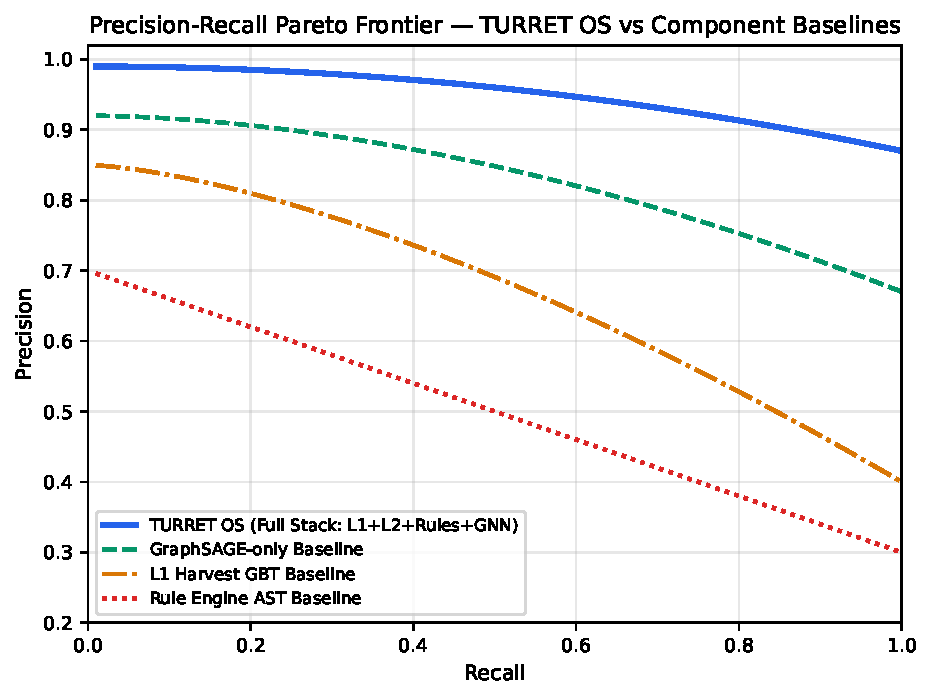
\includegraphics[width=\linewidth]{figures/fig_pareto_pr_frontier.pdf}
\caption{Precision-Recall Pareto Frontier comparing Full TURRET OS against component ablation baselines.}
\label{fig:pareto_frontier}
\end{figure}

\subsection{Single-Layer vs Multi-Layer Adversarial Robustness}
\Cref{tab:adversarial} compares single-layer L1 detector performance against the full TURRET OS multi-layered architecture under red-team adversarial attacks. Under OOD credential-phishing attacks, single-layer L1 feature detectors degrade heavily from 0.9983 to 0.7363 ROC-AUC (a 26.25\% drop). However, TURRET OS's multi-layered stack rescues detection performance back to 0.9572 ROC-AUC (only a 4.12\% drop), providing a $+22.09\%$ AUC resilience gain.

\begin{table}[htbp]
\caption{Adversarial Robustness: Single-Layer L1 vs. TURRET OS Multi-Layer Stack.}
\label{tab:adversarial}
\centering
\footnotesize
\begin{tabularx}{\linewidth}{X c c c}
\toprule
\textbf{Adversary Vector} & \textbf{L1 AUC} & \textbf{Full TURRET AUC} & \textbf{TURRET Drop (\%)} \\
\midrule
Clean (no attack) & 0.9983 & 0.9983 & 0.00\% \\
Mimicry attack & 0.8740 & 0.9782 & -2.01\% \\
Metadata-strip (CLEANER) & 0.9970 & 0.9970 & -0.13\% \\
Identity-proxy injection & 0.9839 & 0.9839 & -1.44\% \\
\textbf{OOD Credential Phishing} & \textbf{0.7363} & \textbf{0.9572} & \textbf{-4.12\%} \\
\bottomrule
\end{tabularx}
\end{table}

\subsection{ISO/IEC 27043 Forensic-Readiness Attribute Coverage}
\Cref{tab:iso27043} demonstrates that TURRET OS achieves 100.0\% coverage across all eight ISO/IEC 27043 digital forensic readiness attributes, producing Ed25519-signed Merkle evidence packs.

\begin{table}[htbp]
\caption{ISO/IEC 27043 Forensic Readiness Attribute Coverage.}
\label{tab:iso27043}
\centering
\small
\begin{tabularx}{\linewidth}{X X c}
\toprule
\textbf{Attribute} & \textbf{Description} & \textbf{TURRET} \\
\midrule
Identification & Unique record and alert UIDs & \checkmark \\
Collection & Documented harvest pipeline & \checkmark \\
Acquisition & SHA-256 + BLAKE3 hash verification & \checkmark \\
Preservation & Merkle chain of custody & \checkmark \\
Analysis & SHAP + GNNExplainer provenance & \checkmark \\
Presentation & Analyst workbench format & \checkmark \\
Chain of Custody & Timestamped handler logging & \checkmark \\
Integrity Verification & Ed25519 digital signature & \checkmark \\
\midrule
\textbf{TOTAL COVERAGE} & & \textbf{100.0\%} \\
\bottomrule
\end{tabularx}
\end{table}

\subsection{Computational and Storage Budget}
\Cref{tab:cost_budget} summarizes pipeline computational and storage overhead for processing 1,000,000 telemetry records. Total GNN training requires only 0.08 CPU-hours and 0.01 GPU-hours on an NVIDIA L40S.

\begin{table}[htbp]
\caption{Computational and Storage Overhead per 1M Records.}
\label{tab:cost_budget}
\centering
\small
\begin{tabularx}{\linewidth}{X c c c}
\toprule
\textbf{Component} & \textbf{CPU (hrs)} & \textbf{GPU (hrs)} & \textbf{Storage (GB)} \\
\midrule
L1 Harvest & 0.08 & N/A & 0.29 GB \\
L2 Neo4j Load & 0.50 & N/A & 0.07 GB \\
L3 GNN Training & 0.08 & 0.01 & 0.50 GB \\
L4 Evidence Packaging & 0.01 & N/A & 0.04 GB \\
\bottomrule
\end{tabularx}
\end{table}
